\section{Referencial Teórico}

\subsection{Aprendizado Infantil}

As crianças passam pelo processo de desenvolvimento e de aprendizagem, muita das vezes estes conceitos são confundidos entre si. O desenvolvimento de uma criança é um processo espontâneo, neste âmbito tem-se o desenvolvimento do corpo, do sistema nervoso, e das funções mentais. O desenvolvimento está relacionado a todas as estruturas do conhecimento. Por outro lado a aprendizagem não é um processo espontâneo, pelo contrário é um processo forçado, localizado apenas em um dos âmbitos do desenvolvimento \cite{piaget:1972}.
Segundo a psicóloga Tharrany de Queiroz Silveira, as crianças começam a desenvolver o raciocínio lógico aproximadamente entre 8 e 12 anos,  sendo que a idade base para este desenvolvimento é aos 10 anos. Mas isso depende do desenvolvimento de cada criança \cite{silveira:2015}.
Mais especificamente, o desenvolvimento de uma criança está dividido em quatro estágio. Cada estágio corresponde a um período do pensamento e do comportamento da criança. Os quatro estágio serão brevemente apresentados abaixo \cite{piaget:1972}:

\begin{itemize}
  \item O \textbf{primeiro estágio}, conhecido como sensório-motor abrange crianças de 0 a 2 anos de idade. Neste estágio é desenvolvido o conhecimento prático, ligado as suas percepções e ao deslocamento do seu corpo. A criança ainda não possui nesta fase uma representação mental, ou seja, os objetos só existem se estiverem no seu campo visual, não existindo assim uma permanência de objetos e imagens em sua cabeça;
  \item O \textbf{segundo estágio}, conhecido como pré-operacional abrange crianças de 2 a 7 anos. Neste estágio surge a formação dos pensamentos, da linguagem, e da representação. Nesta fase tudo o que foi desenvolvido no primeiro estágio (sensório-motor) é transformado em operações, ou seja, as crianças são capazes de criar imagens na ausência física dos objetos. As crianças são capazes de transformar os objetos em outro que lhe traga mais prazer, dar vida aos objetos. Ainda não são capazes de dialogar com outras crianças, ou seja, todos falam ao mesmo tempo, no entanto as frases não apresentam relação uma com as outras;
  \item O \textbf{terceiro estágio}, conhecido como operatório concreto abrange crianças de 7 aos 11/12 anos. Neste estágio a criança desperta o desejo de trabalhar em grupo, a construção da ideia de números, das operações ligadas a lógica elementar bem como de todas as áreas ligadas a exatas (matemática elementar, geometria elementar, e da física elementar). As crianças já são capazes de estabelecer um diálogo, devido ao trabalho em grupo, no entanto ainda não é possível argumentar com pontos de vista distinto para chegarem em uma conclusão final;
  \item O \textbf{quarto estágio}, conhecido como operatório formal, corresponde ao nível do pensamento hipotético-dedutivo abrangendo crianças a partir de 11/12 anos. Neste estágio a criança já é capaz de formar hipóteses, construir novas operações de lógica proposicional, e não apenas a lógica relacionada aos números, é o auge do desenvolvimento da inteligência. As crianças já são capazes de dialogarem entre si, podendo discutir diversos argumentos chegando a uma conclusão final unânime.
\end{itemize}

Em um experimento realizado pela universidade de Mauritius, Husnoo et al. (2013), monitoraram o desempenho de crianças em duas escolas na qual elas desenvolveram atividades utilizando sistemas ICT (information and comunication technology), com base em pré-testes e pós-testes eles verificaram um leve aumento de performance para as crianças que fizeram o teste usando ICT comparado com as que fizeram teste escrito. Também se notou que 75\% das crianças da escola A e 70\% da escola B do experimento, utilizaram a internet para jogar e desenhar. (Cooper \& Brna, 2002) relatam que tecnologia tem sido usada como parte integral do currículo, os estudantes ficam altamente engajados por longos períodos de tempo e demonstram menos problemas comportamentais.

Segundo Druin, 2002; para crianças é mais fácil se expressarem através de desenhos do que por fala e escrita, devido à dificuldade de expressar conteúdos abstratos. Druin (2002) observou que crianças tomam notas mais efetivas de suas observações através de desenhos combinados com pequenas quantidades de textos, do que através de apenas textos descritivos.

De maneira geral, o tempo necessário para realizar tarefas usando estímulo visual foi menor quando comparado ao tempo gasto realizando o pré-teste, como o computador as crianças se tornam aprendizes independentes, entretanto, até mesmo entre as crianças que já possuíam acesso a computadores em casa, os resultados sugerem que as crianças necessitam de ajuda no desenvolvimento das atividades. Através da observação, ficou claro que crianças são capazes de se auto educarem, mas apenas até certo nível. Em suma, crianças usando tecnologia por elas mesmas em um ambiente sem supervisão não é garantia de sucesso e eles irão em algum ponto necessitar de um facilitador \cite{husnoo:2013}.

\subsection{Robótica Educacional}

Segundo José Antônio dos Santos Borges (2011), Robótica Educacional é

“uma atividade desafiadora e lúdica, que utiliza o esforço do educando na criação de soluções de hardware e software visando a resolução de uma situação-problema proposto.”

Segundo Maisonnette (2002), citado por Zilli (2004), a robótica educativa é o controle sobre um mecanismo eletroeletrônico através de um computador. Tais controles são feitos a partir de programas feitos pelo programador, dos quais são interpretados pelo dispositivo para realizar alguma ação.
O uso deste tipo de tecnologia vem levado o ser humano a inovar seu processo de desenvolvimento intelectual a fim de adquirir capacidades de raciocínio de uma forma mais rápida e fácil. A busca por uma melhor compreensão de mundo vem demandado a necessidade de um incremento da capacidade lógica desde a fase infantil. Esta forma de buscar atender as necessidades atuais por conhecimento visam uma maior capacidade de comunicação e aprendizagem por parte do indivíduo.
Um ponto de aceitação entre os educadores é que com o uso de tecnologia o aprendizado torna-se mais dinâmico e interessante para a criança \cite{zilli:2004}. As crianças não adquirem capacidade lógica apenas na escola ou no âmbito familiar, realizar uma ponte entre o uso de ferramentas tecnológicas e os meios normais e tradicionais é de extrema importância e um dos desafios da educação \cite{yus:2004}.
O uso da robótica para desenvolvimento da lógica na criança é uma forma atrativa de ampliar a capacidade de raciocínio. O robô é capaz de auxiliar o entendimento, por parte da criança, de como determinadas ações acontecem e do porquê elas acontecem. A partir disso, os alunos constroem o seu conhecimento com base nas suas experiências e observações gerados pelo esforço próprio. Com isso, o resultado obtido pela criança tem mais significado por se adaptar à sua estrutura mental \cite{zilli:2004}.

Um projeto brasileiro educacional análogo utilizando robôs é o Jabuti Edu. O mesmo projeto visa promover o raciocínio lógico e um contato leve com a programação na educação infantil.  Além do robô conter softwares educacionais,  a plataforma também colabora na aprendizagem de matemática e física. A matemática e a física estão envolvida nas áreas de geometria plana e espacial, álgebra e cinemática. Sobre questão do aprendizado de lógica, os alunos montam um programa que irá simular um experimento de física afim de resolver algum problema.  De acordo com Eloir José Rockenbach, idealizador da comunidade Jabuti Edu “O Jabuti Edu nasce da lacuna que temos na educação infantil para o trabalho com robótica educacional. Ela deveria ser trabalhada em todas as escolas, porque hoje a automação está em todos os lugares e precisamos desenvolver uma cultura digital” \cite{piaget:1985}.

De acordo com Piaget (1985), o conhecimento não acontecerá apenas pela realização práticas na robótica educacional. Em um primeiro momento, tal prática irá desencadear reflexões e diversas áreas de conhecimento, e consequentemente os alunos envolvidos no processo terão a assimilação do conteúdo desejado. Outros conhecimentos poderam ser adquiridos com a integração em grupo no quesito professor e aluno.  No caso do trabalho proposto, as atividades de uso da interface do Raspberry em conjunto ao software educacional implementarão a realidade da robótica na sala de aula e o protagonista de seu aprendizado será os alunos.

\subsection{Iniciativas}

\subsubsection{Scratch}

Projeto liderado pelo grupo Lifelong Kindergarten no Media Lab do MIT. Projetado especialmente para crianças de 8 a 16 anos, porém pode ser usado por usuários de qualquer idade. Iniciado em 2003, o projeto recebe suporte financeiro de instituições como National Science Foundation, Intel Foundation, Dell, Google, do próprio Media Lab do MIT, entre outras.
Em resumo, o Scratch é uma linguagem de programação e uma comunidade online para criação de pequenos projetos, animações, jogos, arte, etc. Ele introduz conceitos matemáticos e computacionais.
As telas disponibilizadas pelo sistema permitem o livre desenho e inserção de dados, e também permite utilizar ilustrações já existentes. Esses desenhos estão ligados à criação desses pequenos projetos, ou sequências animadas para estimular o aprendizado de programação de forma simples e eficiente.
O programa é divido em quatro áreas principais:

\begin{enumerate}
  \item Botões de programação;
  \item Área de programação (comandos, trajes e sons);
  \item Tela de animação;
  \item Hierarquia dos objetos e palco;
\end{enumerate}

Os blocos ou botões de programação estão divididos em categorias: movimento, aparência, som, caneta, controle, sensores, operadores, variáveis.

\begin{figure}[!ht]
\centering
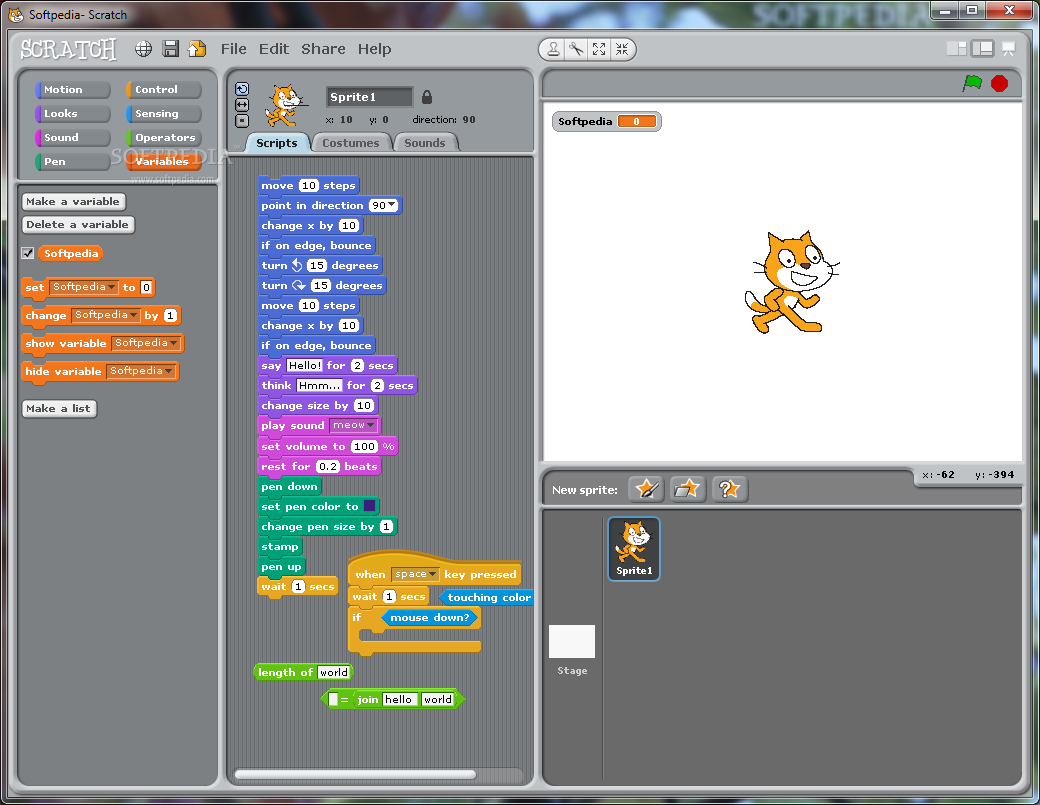
\includegraphics[width=.5\textwidth]{edit/img/scratch.png}
\caption{Captura de Tela - Interface do Scratch}
\label{scratch}
\end{figure}

\subsubsection{Paper Circuits}

O Paper Circuits é um projeto/iniciativa que proporciona aos usuários a construção de pequenos ou complexos circuitos em um pedaço de papel. Em papeis especiais, é possível ligar fitas de cobre e criar cartões, esculturas, origami, ou qualquer outro desenho e adicionar pequenos LEDs nele.
Essa iniciativa é mais uma ferramenta que contribui para a aprendizagem criativa e é embalada pelo movimento cultural dissipada pela internet do DIY, do-it-yourself (faça-você-mesmo, em português).

\begin{figure}[!ht]
\centering
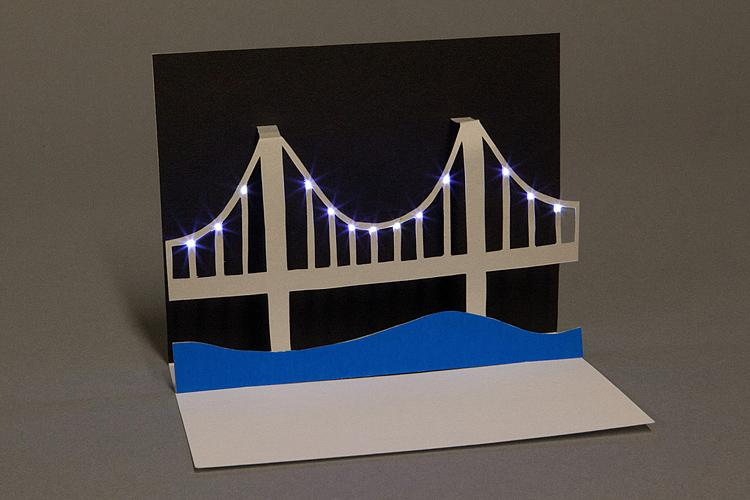
\includegraphics[width=.5\textwidth]{edit/img/circuitpaper.jpg}
\caption{Captura de Tela - Interface do Scratch}
\label{fig:exampleFig1}
\end{figure}

É válido também citar outras iniciativas que estimulam a aprendizagem criativa, são elas:
\begin{itemize}
  \item Caine’s Arcade - A movie that became a movement to foster creativity worldwide;
  \item Intel Computer Clubhouse Network;
  \item The tinkering studio (esse é o espaço que apoia o Paper Circuit e outros projetos);
  \item Transformative Learning Technologies Lab;
  \item Make to Learn;
  \item Maker Camp;
  \item Maker kids.
\end{itemize}

